\section{"Clean Code"}

\subsection{"Pull request", assignation et revue de code}
\begin{figure}[th]
\centering
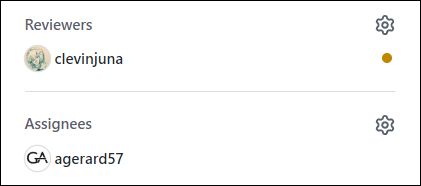
\includegraphics[scale=0.6]{medias/Code_Review_Image.png}
\decoRule
\caption{Exemple de demande de review d'une pull request (Github)}
\end{figure}

Nous créons une "pull request" (ou PR) à chaque branche avec une nouvelle feature/fix/refacto/...., avec une description de la feature.
Une revue de code consiste à étudier les changements effectués dans une branche d'un membre de l'équipe. Cette opération permet d'avoir un oeil neuf sur le code proposé afin de mutuellement s'améliorer.

\subsection{Messages de "commit"}

Tous les messages de commit sont normalisés selon \textbf{Conventional Commits} \parencite{Ref2}. Nous suivons ce pattern afin de mieux comprendre le type / l'utilité / le scope du commit. La transparence est ici vitale pour comprendre plus facilement le code et faciliter le travail des reviewers dans la PR.

\subsection{Convention de nommage}

Un nommage clair des fichiers, des fonctions et des variables dans le code permet de rendre compréhensible un élément du code au premier coup d'oeil, sans pour autant avoir à documenter et expliciter ce que chaque partie du code accomplit.
Par ailleurs, JavaScript et TypeScript obligent, nous avons normalisé le code en "camelCase" pour tout le projet, sauf pour tout ce qui concerne la base de données (snake\_case). Les fonctions ont un contexte plus verbeux, ce qui signifie que tout le temps de réflexion et d'écriture supplémentaire ont pour effet de bord de faire gagner du temps en termes de compréhension ultérieure du code. Enfin, on note que toute la codebase est en anglais (hormis ces rapports de lots). 

\subsection{Une structure solide et rigoureuse}

La rigueur du code et son uniformisation permet de se repérer au mieux. En règle générale, nous faisons en sorte de segmenter notre code de telle façon à ne pas dépasser les 200 lignes par fichier. Pour des cas plus précis:

\subparagraph{/client} Toute notre partie front-end est organisée dans le dossier "\textit{/src} par packages. Ces derniers contiennent tous plus ou moins la même structure.
Cette architecture en packages nous permet de ranger nos imports et exports grâce à la "barrel method" : il s'agit de fichiers index présents dans chaque dossier qui va nous permettre d'y réunir tous nos imports/exports. Lors-ce qu'un composant d'un autre package aura besoin d'un de ces composants exportés, il aura juste à importer sans préciser le fichier en particulier. Cette implémentation est enforcée par eslint, mais nous y reviendrons plus tard (\ref{ESlint}). Enfin, l'utilisation de TypeScript nous oblige à typer l'intégralité de notre code, demandant donc de la régularité. --> \ref{Structure de client et de server}

\subparagraph{/server} Notre back-end a une structure similaire au front, en partie due aux similarités entre JavaScript et TypeScript. Les modèles, contrôleurs, services, routes, etc... sont rangés dans leur packages respectifs. Chaque fichier dans un package correspond à une feature précise. --> \ref{Structure de client et de server}

\subparagraph{/scripts} Ce folder met à disposition des scripts python permettant d'automatiser et donc faciliter nos actions et opérations, comme par exemple la création d'un package template pour client.

\subparagraph{/database} Ce folder est destiné à un usage exclusif aux développeurs, il sert à générer une base de données locale pour mongoDB (afin de faire les tests en environnement local).
Le fichier "index.js" va donc générer la DB, tandit que les fichiers dans /generate vont la peupler avec de la de mock data (en créant par exemple un document Users).

\subparagraph{/docs}
cette partie comprend notre rapport du lot 1, celui du lot 2 et la structure des documents de la base de données. En ce qui concerne la documentation, nous avons aussi donc des commentaires directement dans le code comme mentionné précédemment, mais aussi de la documentation inline sur certaines fonctions indiquant les paramètres, le type attendu ou encore possiblement le comportement de celle-ci.

 
Pour les développeurs, il est mis en place un fichier VS Code \textbf{.workspace} à la racine du repository qui va agencer les différentes parties explicités plus haut.

\subsection{Refléchir avant d'agir}

Un moyen simple mais efficace d'écrire du code convenablement. Évidemment, il se peut que le code ne soit pas parfait, même après une partie conséquente de réflexion. C'est pour cela qu'il faut donc passer assez souvent par une étape de refactoring. Ce concept consiste à retravailler le code de l'application, sans pour autant ajouter de nouvelles fonctionnalités, ni en corriger les éventuelles défaillances.

\subsection{Restrictions Eslint}
\label{ESlint}

Les restrictions d'Eslint imposent d'avantage de normalisation dans la codebase. Nous avons défini quelques règles, comme par exemple l'impossibilité de mettre des "console.log()", l'obligation de ne pas mettre d'accolades dans une fonction ou une condition "if" avec un seul retour, ou l'obligation de camelCase. 

\label{Exemple d'un schéma de validation (Drivers)}
\begin{center}
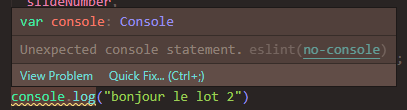
\includegraphics[scale=0.8]{medias/console.png}
\end{center}

\subsection{Utilisation des bons statuts}

A chaque retour d'appel d'api, on envoie le bon statut en fonction de la demande : 200 pour une requête "get", 204 pour "put", 201 pour un "post", 401 pour un "non autorisé", etc. 

\subsection{Commenter, avec partimonie}

Placer des commentaires dans le code est une bonne source de documentation rapide expliquant par exemple le fonctionnement d'un petit bout de code, son résultat attendu, quelques erreurs qui pourraient arriver à cause de celui-ci, etc. Dans notre cas, dû à la clarté du code, peu de commentaires ont été nécessaires. Cependant, il ne faut pas oublier de mentionner certains commentaires très utiles qui ont quand-même trouvé leur place dans notre code, comme ceux qui vont vulgariser des opérations contenant plusieurs opérations "ET" / "OU".


